\chapter*{Management Summary}\addcontentsline{toc}{chapter}{Management Summary}

\textbf{Ausgangslage}

\begin{wrapfigure}{l}{4.5cm}
	\vspace{-0.5cm}
	\begin{center}
		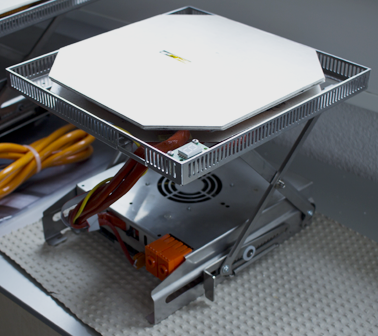
\includegraphics[scale=1]{start/img/img_7680}
	\end{center}
	\vspace{-0.5cm}
\end{wrapfigure}

Die Firma \fluxron{} entwickelt und produziert in Amriswil Heizlösungen und Küchengeräte mit Induktionstechnologie. Die Küchengeräte sind allerdings keine Produkte für die private Küche zuhause, sondern Einbaugeräte für Kombinationen in Grossküchen. Darunter sind neben verschiedenen Induktionsherdmodellen auch elektronisch gesteuerte Thermostate. Meistens werden die Geräte nicht durch Fluxron selbst verbaut, sondern über eine Servicefirma installiert und dann beim Endkunden in der Grossküche verbaut.

Fluxron stattet die Geräte serienmässig mit einem Bluetoothmodul aus. Darüber können ohne Kabelverbindung die Geräteeinstellungen angepasst und ausgelesen werden. Zudem liefert die Schnittstelle auch ausführliche Laufzeit- und Fehlerprotokolle.

\begin{wrapfigure}{r}{4.5cm}
	\vspace{-0.5cm}
	\begin{center}
		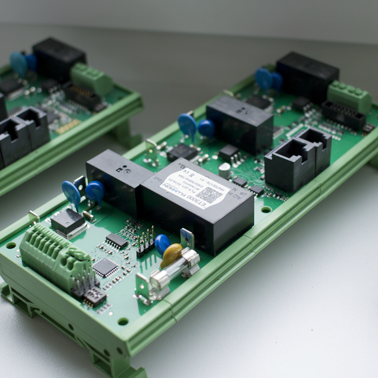
\includegraphics[scale=1]{start/img/img_7689}
	\end{center}
	\vspace{-0.5cm}
\end{wrapfigure}

Ein Servicetechniker benötigt genau diese Informationen, um vor einer allfälligen Reparatur der Geräte in Grossküchen eine Diagnose des Problems zu stellen. Dies ist besonders nützlich, da häufig keine Reparatur des Gerätes nötig ist, sondern nur eine Einstellung geändert werden muss. Oft wird Vielzahl von Geräten verbaut und es ist für die Techniker schwierig, die Installationen auch bei einem späteren Serviceeinsatz noch genau zu kennen. Sie sollen dabei durch eine Smartphone Applikation unterstützt werden.

Die Firma hat bereits eine solche Applikation im Einsatz, allerdings kann diese nur für den Gebrauch mit einem einzelnen Gerät genutzt werden. Daher soll eine neue App von Grund auf entwickelt werden. Damit sollen Techniker die Installationen in den verschiedenen Küchen speichern, und bei der Wartung wieder abrufen können. Sie sollen die Geräte in einem Suchlauf finden, deren Position in der Küche markieren und den Status einsehen können. Weiter soll es möglich sein die Einstellungen der Geräte mit der App anzupassen.

\textbf{Vorgehen}

Zur Umsetzung des Projektes wurden agile Softwareentwicklungsmethoden eingesetzt. In  wöchentlichen Meetings wurde die weiteren Aufgaben priorisiert und in planbare Tasks aufgeteilt. Initialisiert wurde das Projekt mit einer gründlichen Anforderungsanalyse mittels User Stories und Use Cases. 

Aufbauend auf den Anforderungen wurde dann die Benutzeroberfläche mittels Mockups entworfen und im Walkthrough besprochen. Dies lieferte die Grundlage für die technische Konzeption der Applikation, welche aus der Architekturdefinition und Evaluationen zur genutzten Technologie besteht.

Nach Analyse und Konzeption wurde die Anwendung iterativ im Wochenrhythmus implementiert und getestet. Um die korrekte Funktionsweise zu garantieren, wurde die App nochmals vor Ort mit vollständigen Geräteinstallationen erfolgreich getestet.

\begin{wrapfigure}{r}{4cm}
	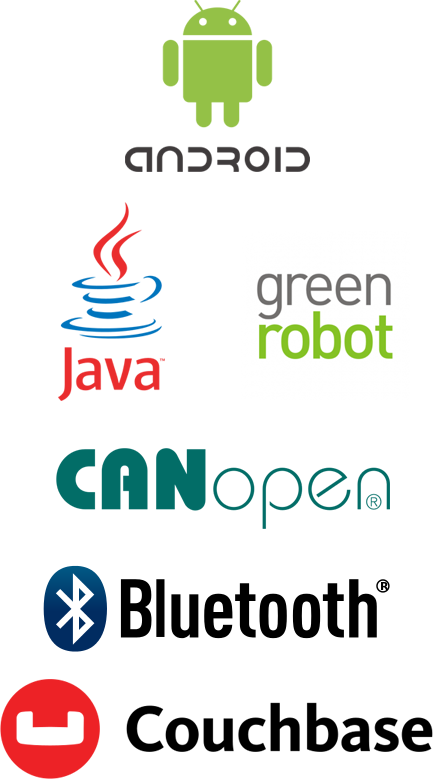
\includegraphics[scale=0.26]{start/img/logos}
\end{wrapfigure}
\textbf{Technologien}

Bild des Technologiestacks (Icons der Hersteller).

Die Anwendung wurde mit Java 7 für Android umgesetzt. Um eine gute Kompatibilität zu gewährleisten, ist die App ab Androidversion 4.3 und höher nutzbar. Die Anwendungsarchitektur besteht aus drei Ebenen, welche mittels Meldungen über den Green Robot Event Bus kommunizieren.

Alle Anwendungsdaten werden in einer lokalen Couchbase Lite-Datenbank gespeichert und können über die Exportfunktion per EMail ausgetauscht werden. Die Kommunikation mit der Hardware erfolgt über das CANopen-Protokoll und funktioniert somit für alle Küchengeräte der Firma Fluxron.

\begin{wrapfigure}{r}{4.5cm}
	\vspace{-1.1cm}
	\begin{center}
		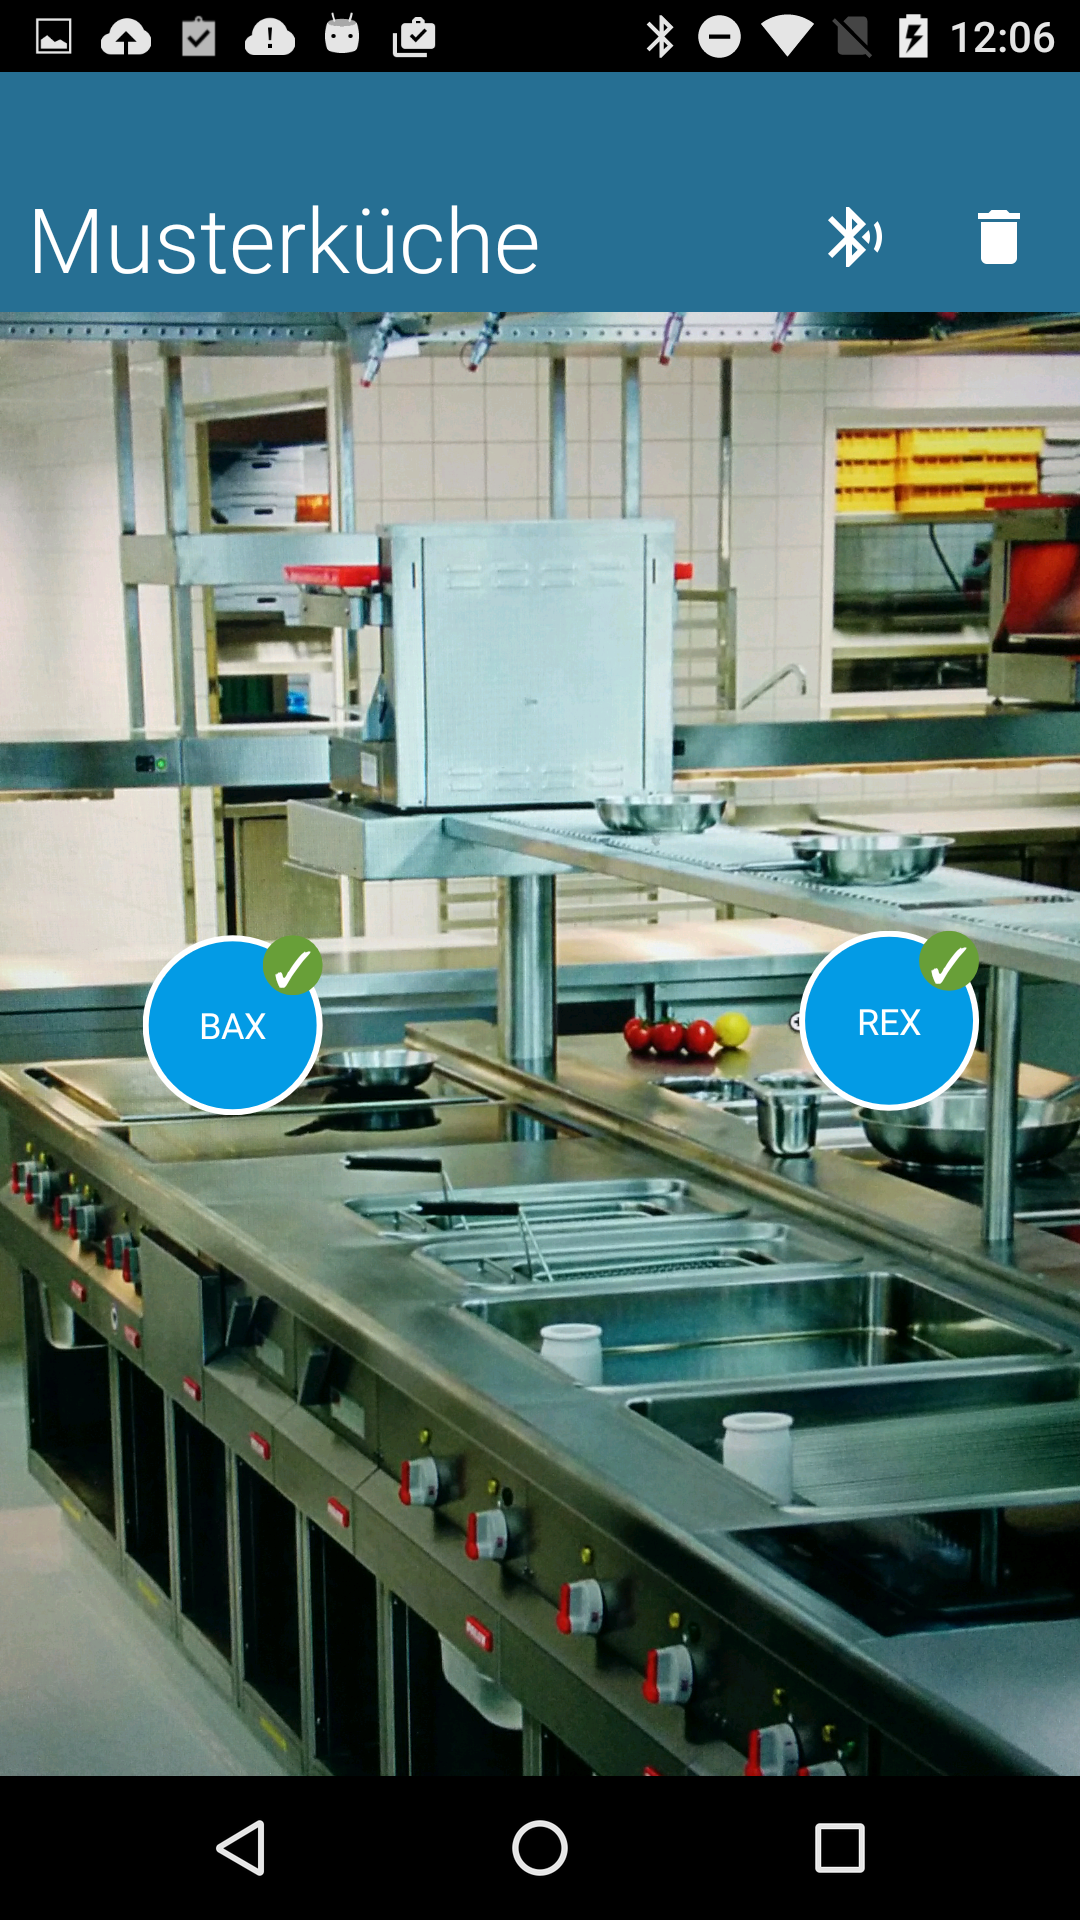
\includegraphics[scale=0.12]{start/img/screenshot}
	\end{center}
	\vspace{-1cm}
\end{wrapfigure}

\textbf{Ergebnisse}

Die Anwendung unterstützt das Erfassen einer beliebigen Anzahl von Küchen. Der Techniker kann für jede Installation eine eigen Küche erfassen und diese einfach über die Suchfunktion wieder finden. Küchen können um zusätzliche Beschreibungen ergänzt werden.

Um die Situation in einer Grossküche genau erfassen zu können, kann der Techniker die Küche in verschiedene Bereiche unterteilen. Diese werden jeweils mit einem Foto hinterlegt und sind so einfach und effizient erfasst.

Damit die Servicetechniker die genauen Positionen der eingebauten Geräte auch später bei einem Wartungsauftrag noch kennen, können die aktiven Geräte mit einem Suchlauf aufgelistet und auf einem Küchenbereich platziert werden.
\WFclear

Für Servicezwecke kann nun ohne Ausbau oder direkten Zugang zu den Geräten der Status abgefragt werden. Der Techniker sieht auf einen Blick alle Sensorwerte und kann sich die Fehlerprotokolle und Statuszähler anzeigen lassen.\\
\begin{wrapfigure}{l}{4.5cm}
	\vspace{-.5cm}
	\begin{center}
		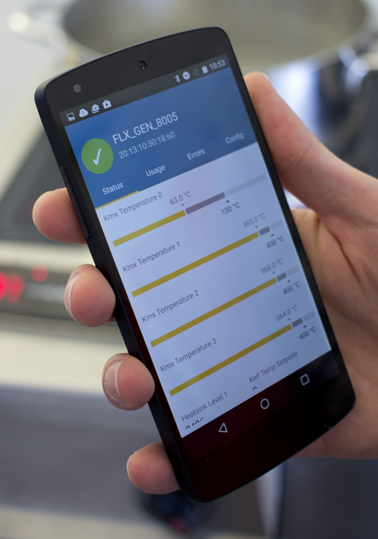
\includegraphics[scale=1]{start/img/img_7610}
	\end{center}
	\vspace{-1cm}
\end{wrapfigure}
Die Werte werden durch die Applikation für alle Geräte automatisch aktualisiert und ermöglichen somit ein effizientes Arbeiten, auch bei der Diagnose von Problemen bei verschiedenen Geräten ist nur wenig manuelle Interaktion notwendig.

Damit wird das Problem der umständlichen Diagnose und Wartung der Geräte gelöst. Die Techniker erfassen die Situation der Küche bereits bei der Installation und können dann bei der Wartung diese wieder abrufen. Dabei ist kein manueller Verbindungsaufbau mehr nötig, da die Geräte bereits erfasst sind.

\pagebreak

\textbf{Ausblick}

Die Anwendung wird nun an die Firma Fluxron übergeben und dort zur Marktreife weiterentwickelt und von Servicefirmen und Technikern der Firma Fluxron verwendet.

In der aktuellen Version der App wurden aus Zeitgründen nur die Gerätetypen C- und S-Class vollständig angebunden. Es ist aber problemlos möglich, weitere Fluxron-Geräte anzusprechen. Die Anwendung unterscheidet die Geräte bereits an ihrem Herstellercode und kann daher um beliebige Gerätetypen erweitert werden. Es muss lediglich die Benutzeroberfläche für die entsprechenden Gerätetypen definiert werden. Neben der Oberfläche kann auch ein neuer Parametersatz (EDS-Datei) integriert werden. Dieser wird dann über die automatische Generierung für den Entwickler vorbereitet und kann einfach mit der Benutzeroberfläche verbunden werden.

Neben neuen Gerätetypen bietet die Anwendung noch weiteres Potenzial für die Zukunft. So könnte zum Beispiel eine Funktion zum Einlesen und Versenden der gesamten Gerätekonfiguration neue Möglichkeiten bei Diagnose und Konfiguration bieten.

Ausserdem ist die App bereits jetzt darauf vorbereitet, an die Cloud angebunden zu werden. Dies einerseits durch die Verwendung einer entsprechenden Datenbanktechnologie und andererseits durch die meldungsbasierte Architektur. Damit würden sich neue Möglichkeiten wie z.B. Nutzungs- oder Fehlerprotokolle bieten. Zudem könnten die Servicefirmen damit alle Küchen zentral speichern und müssten die Küchen nicht mehr per EMail verteilen.

\vspace{1.4cm}

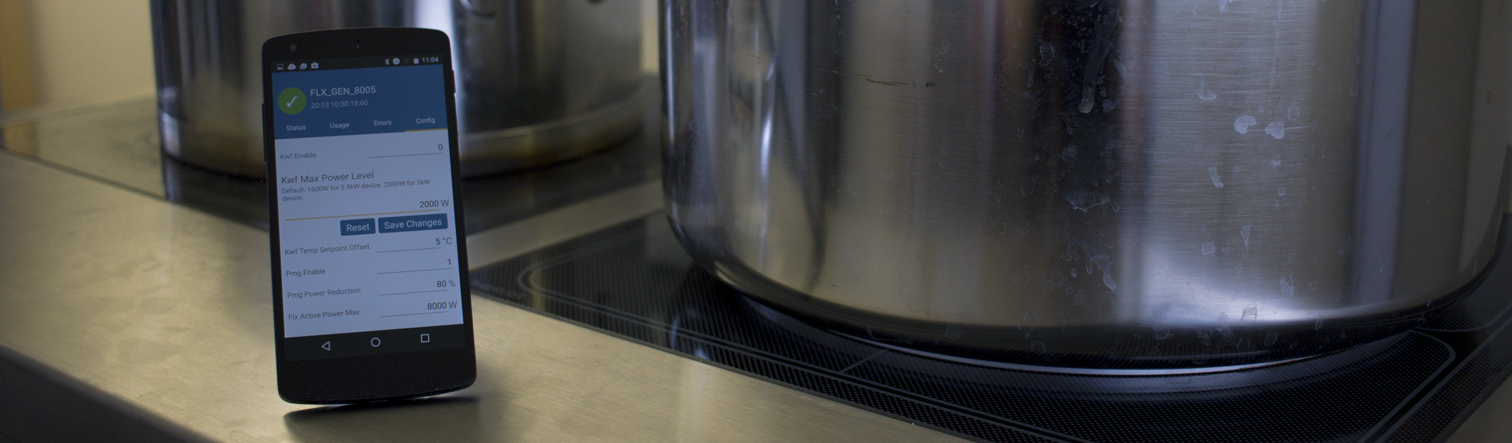
\includegraphics[trim={0 0 36 0},clip]{start/img/img_7670}